\documentclass{article}

% NeurIPS 2025 style -- final version
\usepackage[main, final]{neurips_2025}

\usepackage[utf8]{inputenc}
\usepackage[T1]{fontenc}
\usepackage{hyperref}
\usepackage{url}
\usepackage{booktabs}
\usepackage{amsfonts}
\usepackage{amsmath}
\usepackage{nicefrac}
\usepackage{microtype}
\usepackage{xcolor}
\usepackage{graphicx}
\usepackage{subcaption}
\usepackage{multirow}
\usepackage{enumitem}

% ── Tighter spacing ──
\setlength{\textfloatsep}{8pt plus 2pt minus 2pt}
\setlength{\floatsep}{6pt plus 1pt minus 1pt}
\setlength{\intextsep}{6pt plus 1pt minus 1pt}
\setlength{\abovecaptionskip}{4pt}
\setlength{\belowcaptionskip}{2pt}
\setlist{nosep, leftmargin=*}

\title{Data-Driven Revenue Analytics and Forecasting\\for Vietnamese E-Commerce Fashion}

\author{
  Duong Phuong Thao \quad
  Nguyen Nang Anh \quad
  Hoang Ngoc Anh \quad
  Trinh Thi Thuy Duong
}

\begin{document}
\maketitle
\vspace{-0.3cm}

% ==============================================================================
% ABSTRACT
% ==============================================================================
\begin{abstract}
We present an analytics and forecasting framework for a Vietnamese e-commerce fashion enterprise, analyzing 15 datasets spanning 3,833 days (Jul~2012--Dec~2022). Our contributions: (1)~a four-level framework (Descriptive$\to$Diagnostic$\to$Predictive$\to$Prescriptive) across five business themes, revealing traffic-driven seasonality, stagnant AOV, and 29\% customer churn risk; and (2)~an ensemble forecasting pipeline (XGBoost+LightGBM+CatBoost) with recursive day-by-day prediction, 63 features from Fourier harmonics, lag/rolling statistics, and Vietnamese event markers. The pipeline achieves the best Kaggle leaderboard score among six experimental versions. SHAP analysis confirms lag features and cyclical encodings as dominant predictors. Code: \url{https://github.com/thao12345310/datathon-2026-hkt}
\end{abstract}

% ==============================================================================
% SECTION 1: DATA EXPLORATION & ANALYSIS
% ==============================================================================
\section{Data Exploration \& Analysis}

We analyze 15 CSV files ($\sim$130M rows) from a Vietnamese fashion e-commerce company. For each business theme, we apply a four-level framework: \textbf{Descriptive} (what happened?), \textbf{Diagnostic} (why?), \textbf{Predictive} (what will happen?), and \textbf{Prescriptive} (what should we do?).

\subsection{Revenue Seasonality \& Trend Decomposition}

\textbf{Descriptive.} Total revenue is 16.43B VND over 2012--2022 (avg.\ 4.29M/day). The business follows an inverted-U lifecycle: growth to a 2.10B peak in 2016, decline through 2021 ($-38.6\%$ YoY in 2019), and recovery in 2022 ($+12.1\%$). Q2 (Apr--Jun) averages 152\% of the overall mean; Q4 (Oct--Dec) only 66\%.

\textbf{Diagnostic.} Decomposing $\text{Revenue} = \text{Sessions} \times \text{Conversion} \times \text{AOV}$: Q2 sessions are $+111\%$ vs.\ Q4, while AOV differs only $+15\%$. Critically, Q4 conversion (0.78\%) is \emph{higher} than Q2 (0.72\%)---the weakness stems from visitor volume, not purchase intent. Revenue correlates strongly with order count ($r = 0.93$) but only moderately with sessions ($r = 0.46$).

\textbf{Predictive.} The \emph{direction} of seasonality (Q2$>$Q4) is stable across all years, but the \emph{magnitude} is not: monthly coefficient of variation is 25--35\%, with peak months declining from $\sim$200\% index (2015--18) to $\sim$105\% (2019--22).

\textbf{Prescriptive.} (1)~Plan Q2 inventory conservatively at 120--130\%, not historical 200\%. (2)~Investigate Q4 traffic drop root cause before increasing marketing spend. (3)~Verify Tet-period fulfillment capacity before promotions.

\subsection{Customer Segmentation \& Lifetime Value}

Analysis of 90,246 customers: the 25--44 age group contributes 55.8\% of total revenue. All six acquisition channels yield nearly identical customer quality ($<$3\% variation), suggesting \emph{volume} optimization over channel selection. AOV has remained flat at $\sim$24K VND for 10 years---a significant missed upsell opportunity.

\textbf{Churn analysis.} Using recency-to-gap ratio thresholds, 29.1\% of repeat customers (19,770) are classified as \textbf{High Risk} ($>$3$\times$ their average inter-order gap), representing 3.74B VND in at-risk revenue. Combined Medium+High Risk: 5.64B VND (36\% of repeat-customer revenue). Priority action: win-back campaigns targeting 8,271 Medium Risk customers with estimated ROI of 10--20$\times$.

\subsection{Promotion Effectiveness \& Geographic Concentration}

$\sim$39\% of order items have associated promotions. Promotional orders show slightly lower return rates, but AOV impact is minimal due to discount absorption. The \textbf{East region} accounts for 46.5\% of total revenue, creating vulnerability to regional disruptions.

\begin{figure}[t]
  \centering
  \begin{subfigure}[b]{0.32\linewidth}
    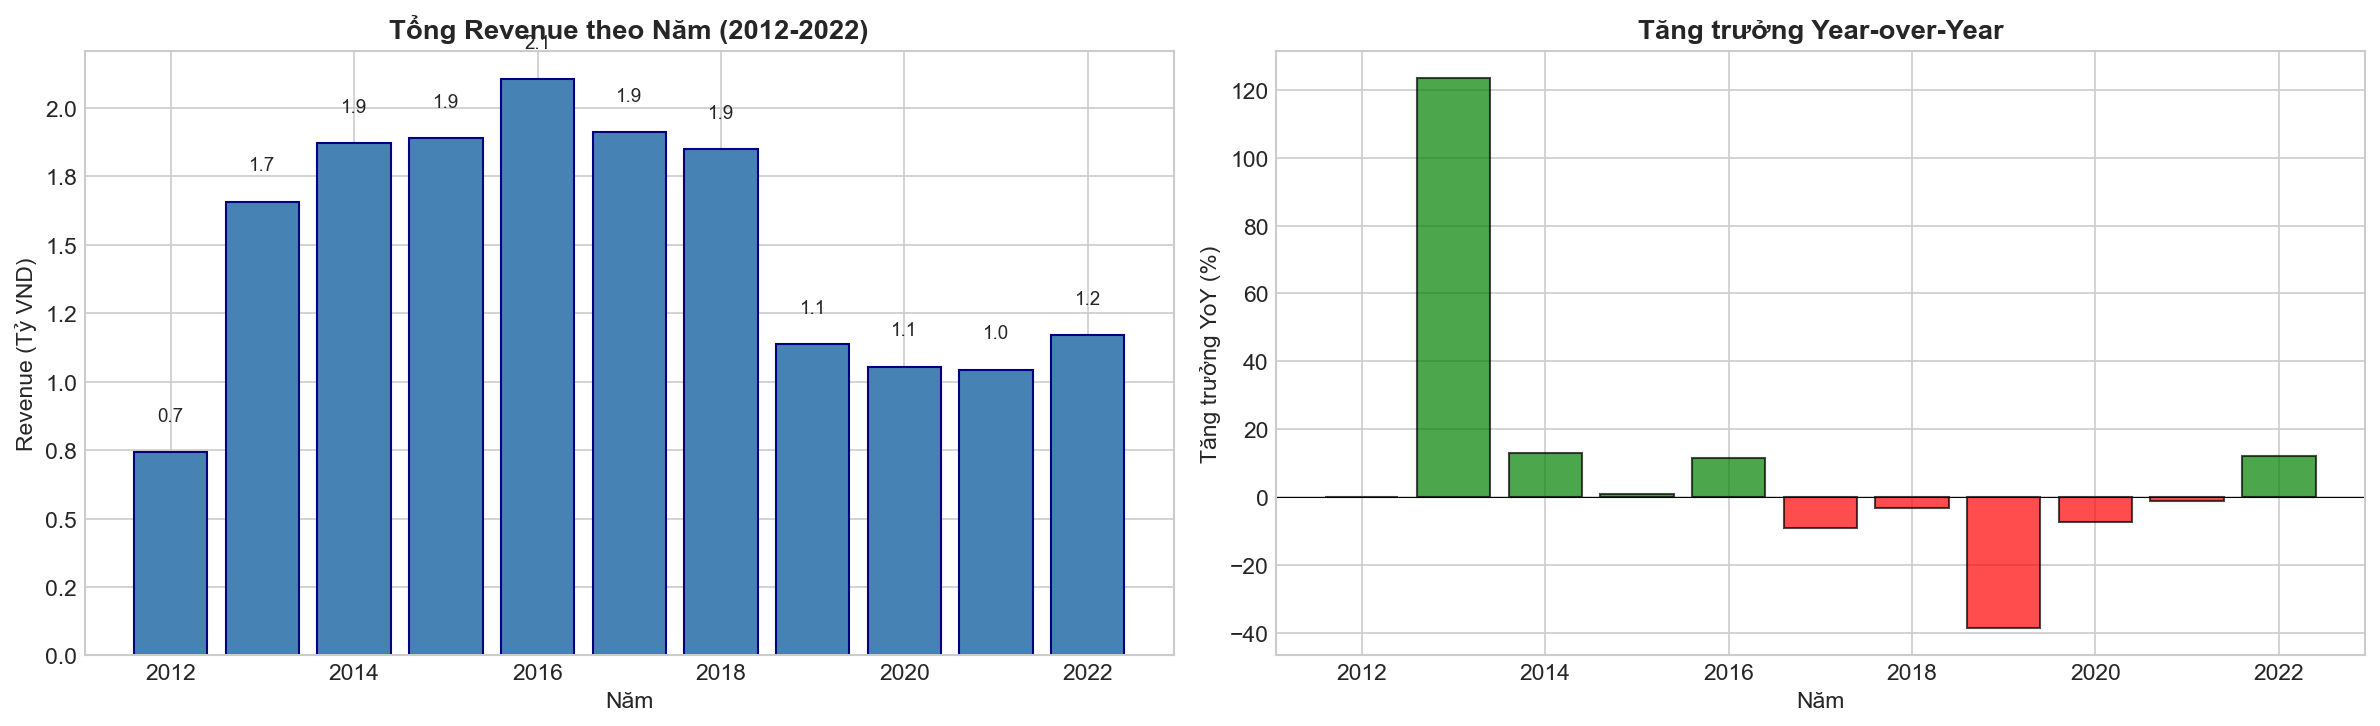
\includegraphics[width=\linewidth]{figures/BAO_CAO_CHU_DE1/revenue_by_year.png}
    \vspace{-0.5cm}
    \caption{Annual revenue trend}
    \label{fig:rev_year}
  \end{subfigure}
  \hfill
  \begin{subfigure}[b]{0.32\linewidth}
    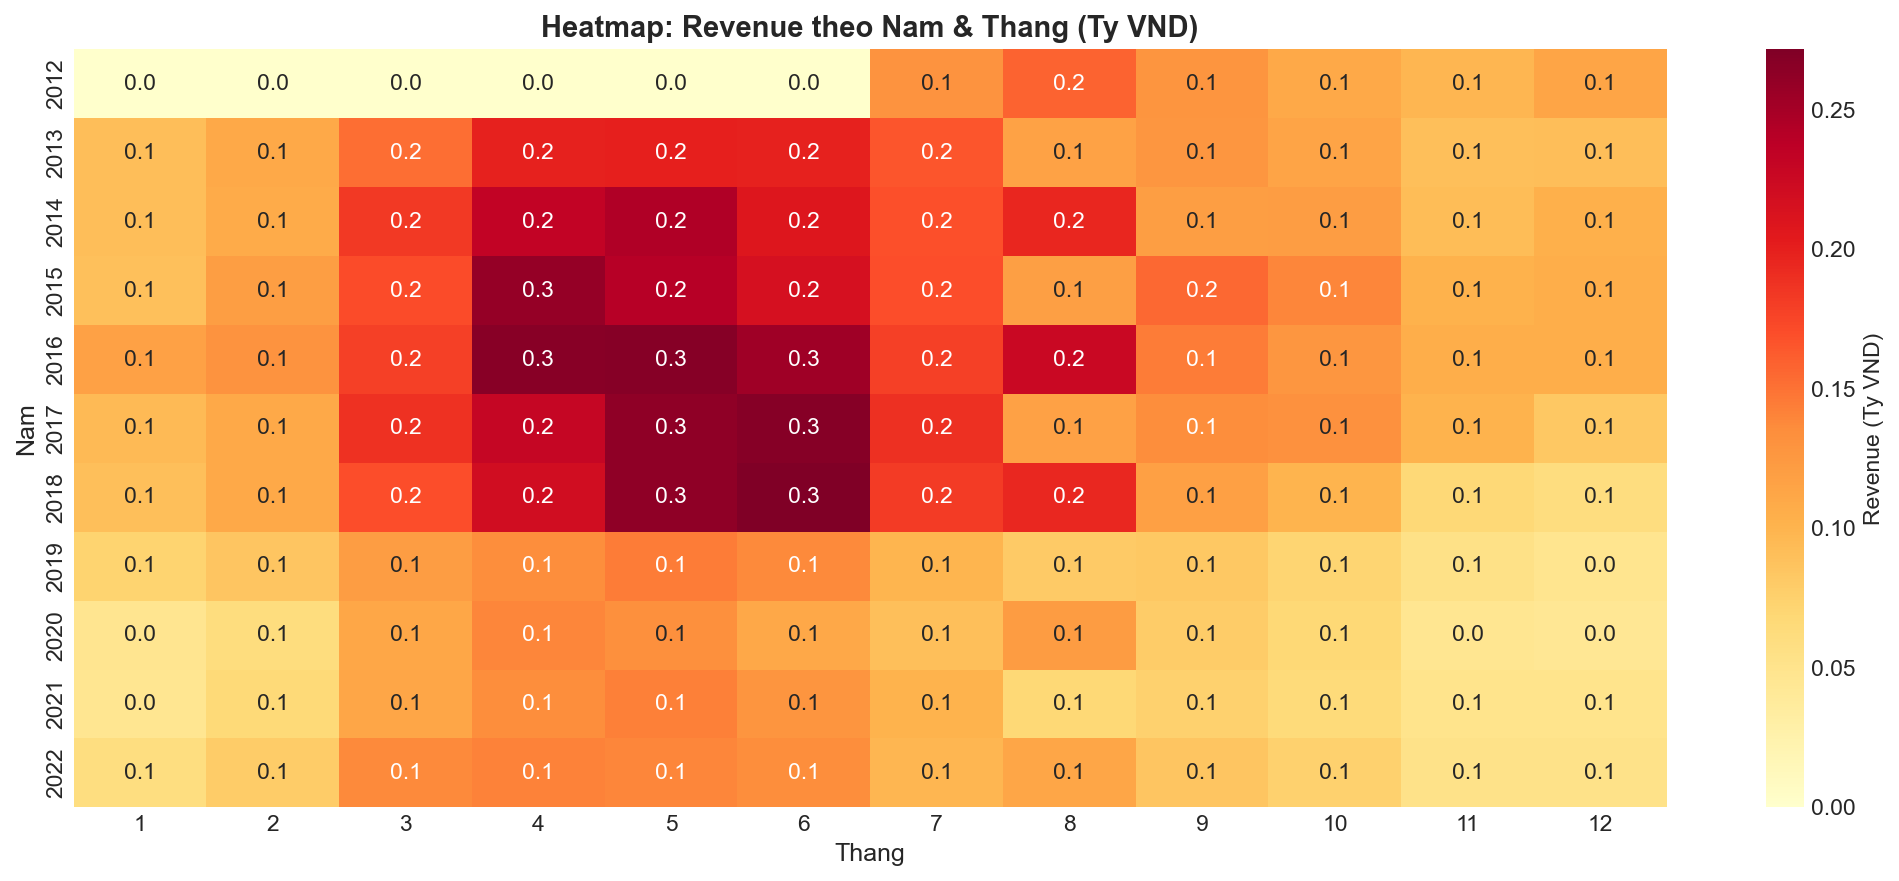
\includegraphics[width=\linewidth]{figures/BAO_CAO_CHU_DE1/revenue_heatmap.png}
    \vspace{-0.5cm}
    \caption{Monthly heatmap}
    \label{fig:rev_heatmap}
  \end{subfigure}
  \hfill
  \begin{subfigure}[b]{0.32\linewidth}
    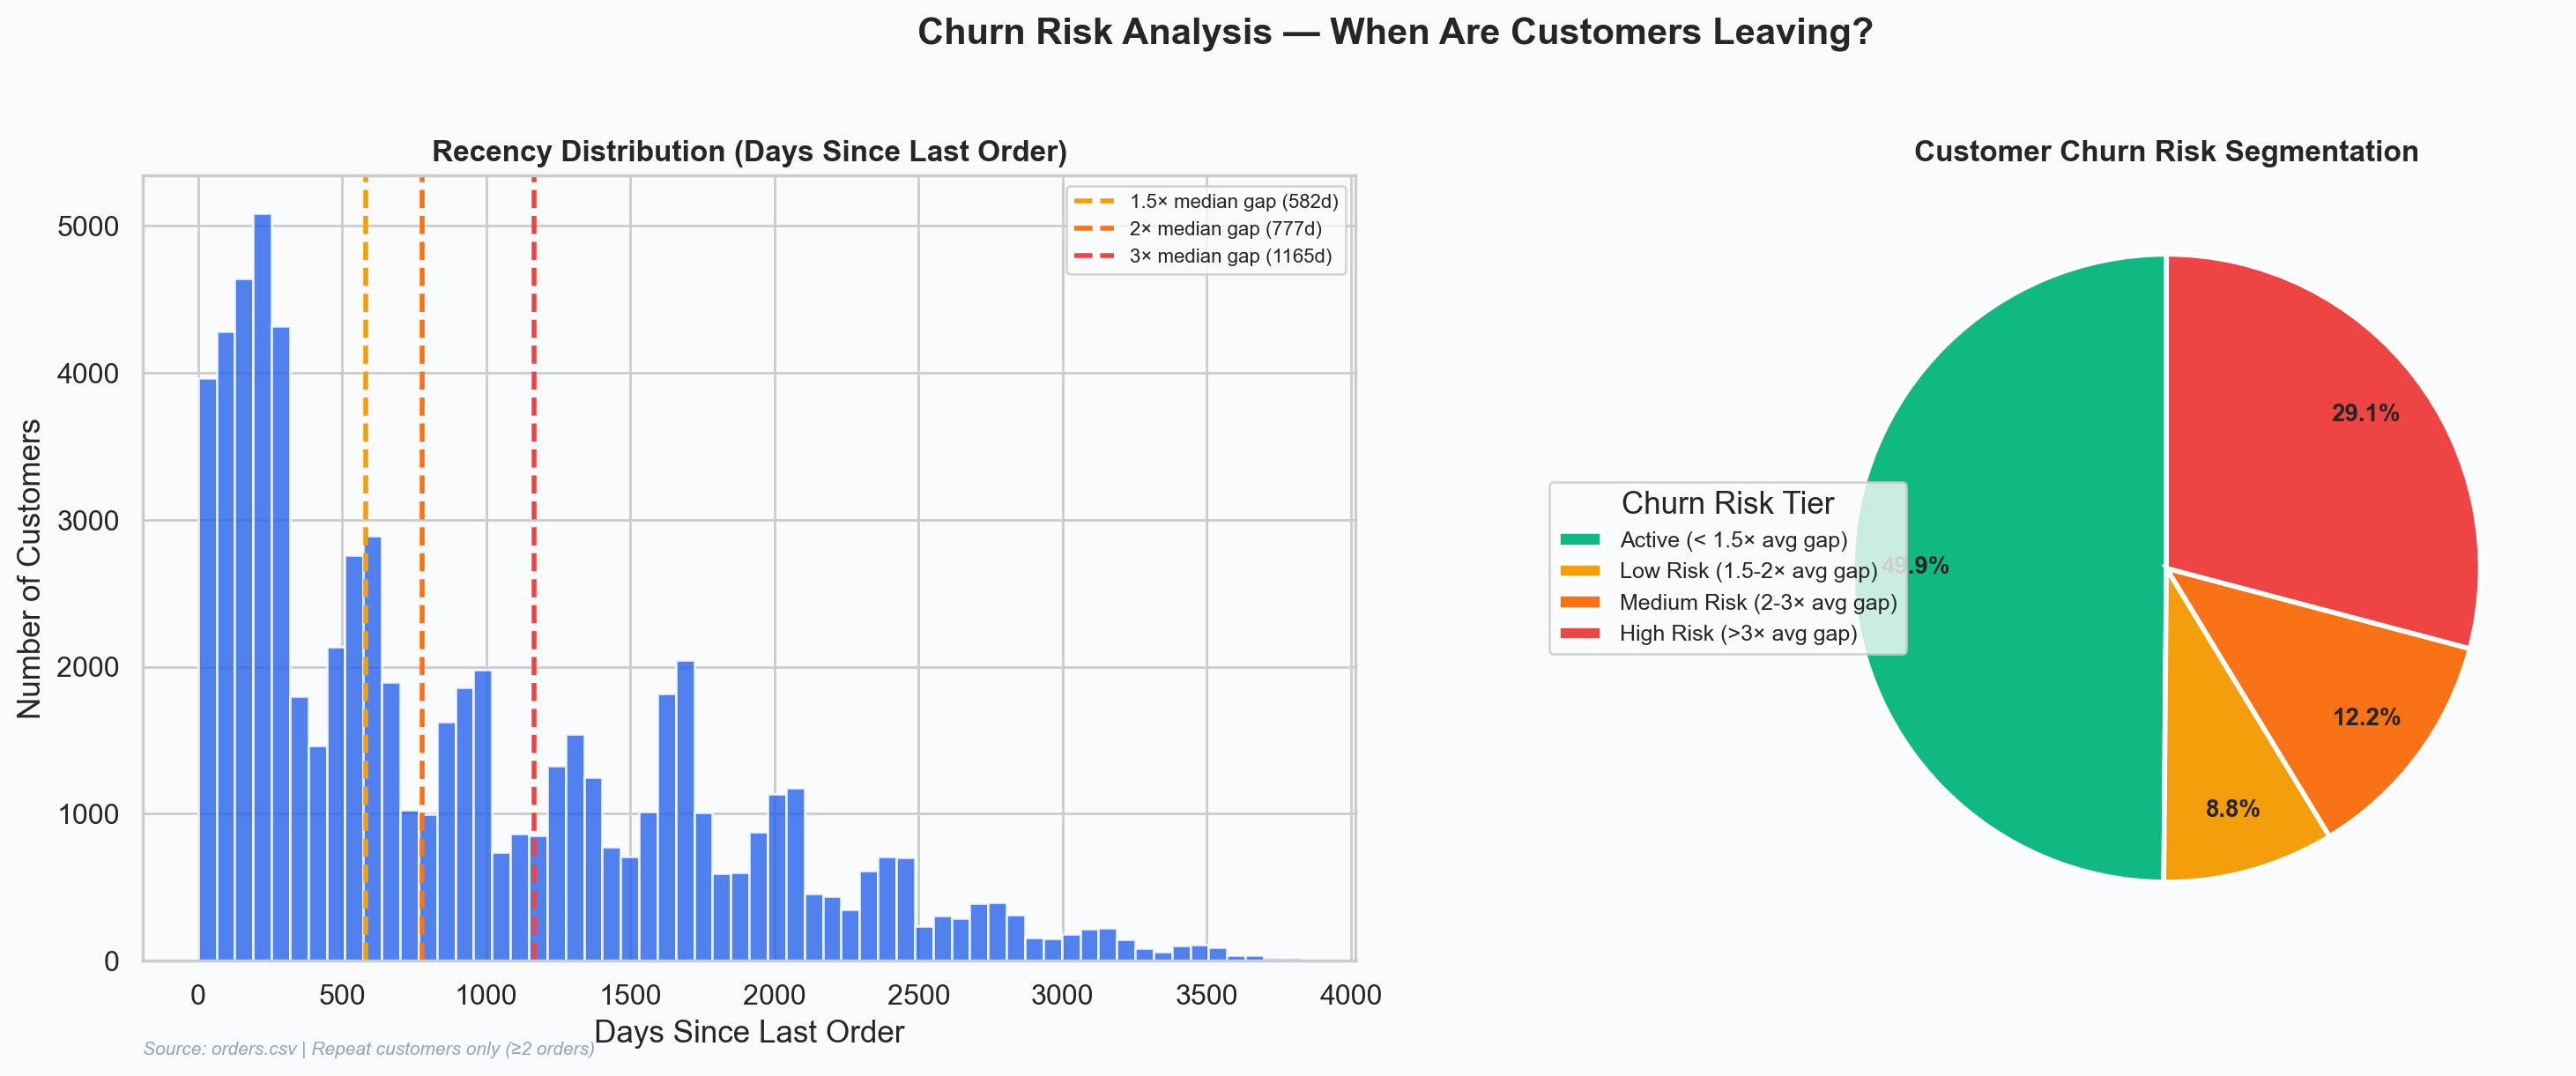
\includegraphics[width=\linewidth]{figures/story2_chart4_churn_risk.png}
    \vspace{-0.5cm}
    \caption{Churn risk distribution}
    \label{fig:churn}
  \end{subfigure}
  \vspace{-0.1cm}
  \caption{(a)~Inverted-U revenue lifecycle with 2022 recovery. (b)~Q2 dominates consistently; magnitude declines post-2018. (c)~29.1\% of repeat customers at high churn risk (3.74B VND at stake).}
  \label{fig:eda}
\end{figure}


% ==============================================================================
% SECTION 2: FORECASTING METHODOLOGY
% ==============================================================================
\section{Forecasting Methodology}

\textbf{Task.} Forecast daily Revenue and COGS for 548 test days (Jan~2023--Jul~2024) given 3,833 training days.

\subsection{Feature Engineering (63 Features)}

We construct features in five categories (Table~\ref{tab:features}). A key design choice: rely \emph{solely} on the target series and calendar---external signals (web traffic, inventory) proved noisy in later experiments and hurt Kaggle generalization.

\begin{table}[t]
  \caption{Feature categories. All lags use \texttt{shift(1)} to prevent leakage.}
  \label{tab:features}
  \centering
  \small
  \begin{tabular}{lcp{5.8cm}}
    \toprule
    \textbf{Category} & \textbf{\#} & \textbf{Description} \\
    \midrule
    Calendar & 10 & Year, month, quarter, DoW, DoM, DoY, WoY, weekend, month start/end \\
    Cyclical / Fourier & 16 & Sin/cos for month, DoW, DoY; annual harmonics $k\!\in\!\{1,2,3,4,6\}$; weekly harmonics $k\!\in\!\{1,2,3\}$ \\
    Vietnamese events & 5 & Tet, 11/11, 12/12, year-end, Black Friday \\
    Lag features & 11 & $\{1,2,3,7,14,21,28,30,60,90,365\}$ days \\
    Rolling / expanding & 21 & Mean/std/min/max at $\{7,14,30,60,90\}$d; expanding mean; 1d \& 7d diffs \\
    \bottomrule
  \end{tabular}
\end{table}

Fourier harmonics encode annual and weekly seasonality non-parametrically. A linear trend index (\texttt{trend\_idx}) allows the model to capture long-term revenue decline. Rows with missing \texttt{lag\_365} are dropped, yielding $\sim$3,468 usable training samples.

\subsection{Model Architecture \& Cross-Validation}

We ensemble three gradient-boosted tree algorithms, averaging their outputs (clipped $\geq 0$): \textbf{XGBoost}~[2] ($n_\text{est}\!=\!2000$, depth$\!=\!7$, $\eta\!=\!0.02$, subsample$\!=\!0.8$, colsample$\!=\!0.7$, $\alpha\!=\!0.5$, $\lambda\!=\!2.0$), \textbf{LightGBM}~[3] (identical, leaf-wise growth), and \textbf{CatBoost}~[4] ($\text{iter}\!=\!2000$, depth$\!=\!7$, $\ell_2\!=\!5.0$). All use \texttt{seed=42}. During CV, early stopping (50 rounds) is enabled with $n_\text{est}\!=\!1500$ and $\eta\!=\!0.03$; final models use full data.

\begin{table}[t]
  \caption{5-fold TimeSeriesSplit cross-validation results}
  \label{tab:cv}
  \centering
  \small
  \begin{tabular}{lcc|cc}
    \toprule
    & \multicolumn{2}{c|}{\textbf{Revenue}} & \multicolumn{2}{c}{\textbf{COGS}} \\
    \textbf{Model} & MAE & $R^2$ & MAE & $R^2$ \\
    \midrule
    XGBoost  & \textbf{737,579} & \textbf{0.814} & \textbf{621,122} & \textbf{0.813} \\
    LightGBM & 747,050 & 0.808 & 643,204 & 0.804 \\
    CatBoost & 786,094 & 0.787 & 678,017 & 0.780 \\
    \bottomrule
  \end{tabular}
\end{table}

\textbf{Why simplicity wins.} Later versions (v3--v6) added external signals, multi-seed ensembles (9 models), and EWM features, achieving CV $R^2 > 0.93$. However, v2's simpler pipeline produced the best \emph{Kaggle leaderboard} score. For 548-day recursive forecasting, feature parsimony avoids compounding errors from noisy external inputs---a clear demonstration of the bias--variance tradeoff.

\subsection{Recursive Prediction \& SHAP Interpretability}

For each test day $t$: (1)~append a placeholder to history; (2)~rebuild all features from the full history including prior predictions; (3)~average the three model outputs; (4)~write back to history. This ensures lag/rolling feature consistency over the 18-month horizon without any post-hoc drift correction.

SHAP TreeExplainer~[5] on the XGBoost component identifies \texttt{lag\_1}, \texttt{rmean\_7}, \texttt{doy\_sin}, \texttt{lag\_7}, and \texttt{rmean\_30} as the top-5 features (Figure~\ref{fig:results}b). This confirms reliance on two information sources: \emph{short-term momentum} (lags, rolling means) and \emph{annual cyclicality} (Fourier)---consistent with EDA seasonality findings and explaining why the simple feature set generalizes well.

\begin{figure}[t]
  \centering
  \begin{subfigure}[b]{0.52\linewidth}
    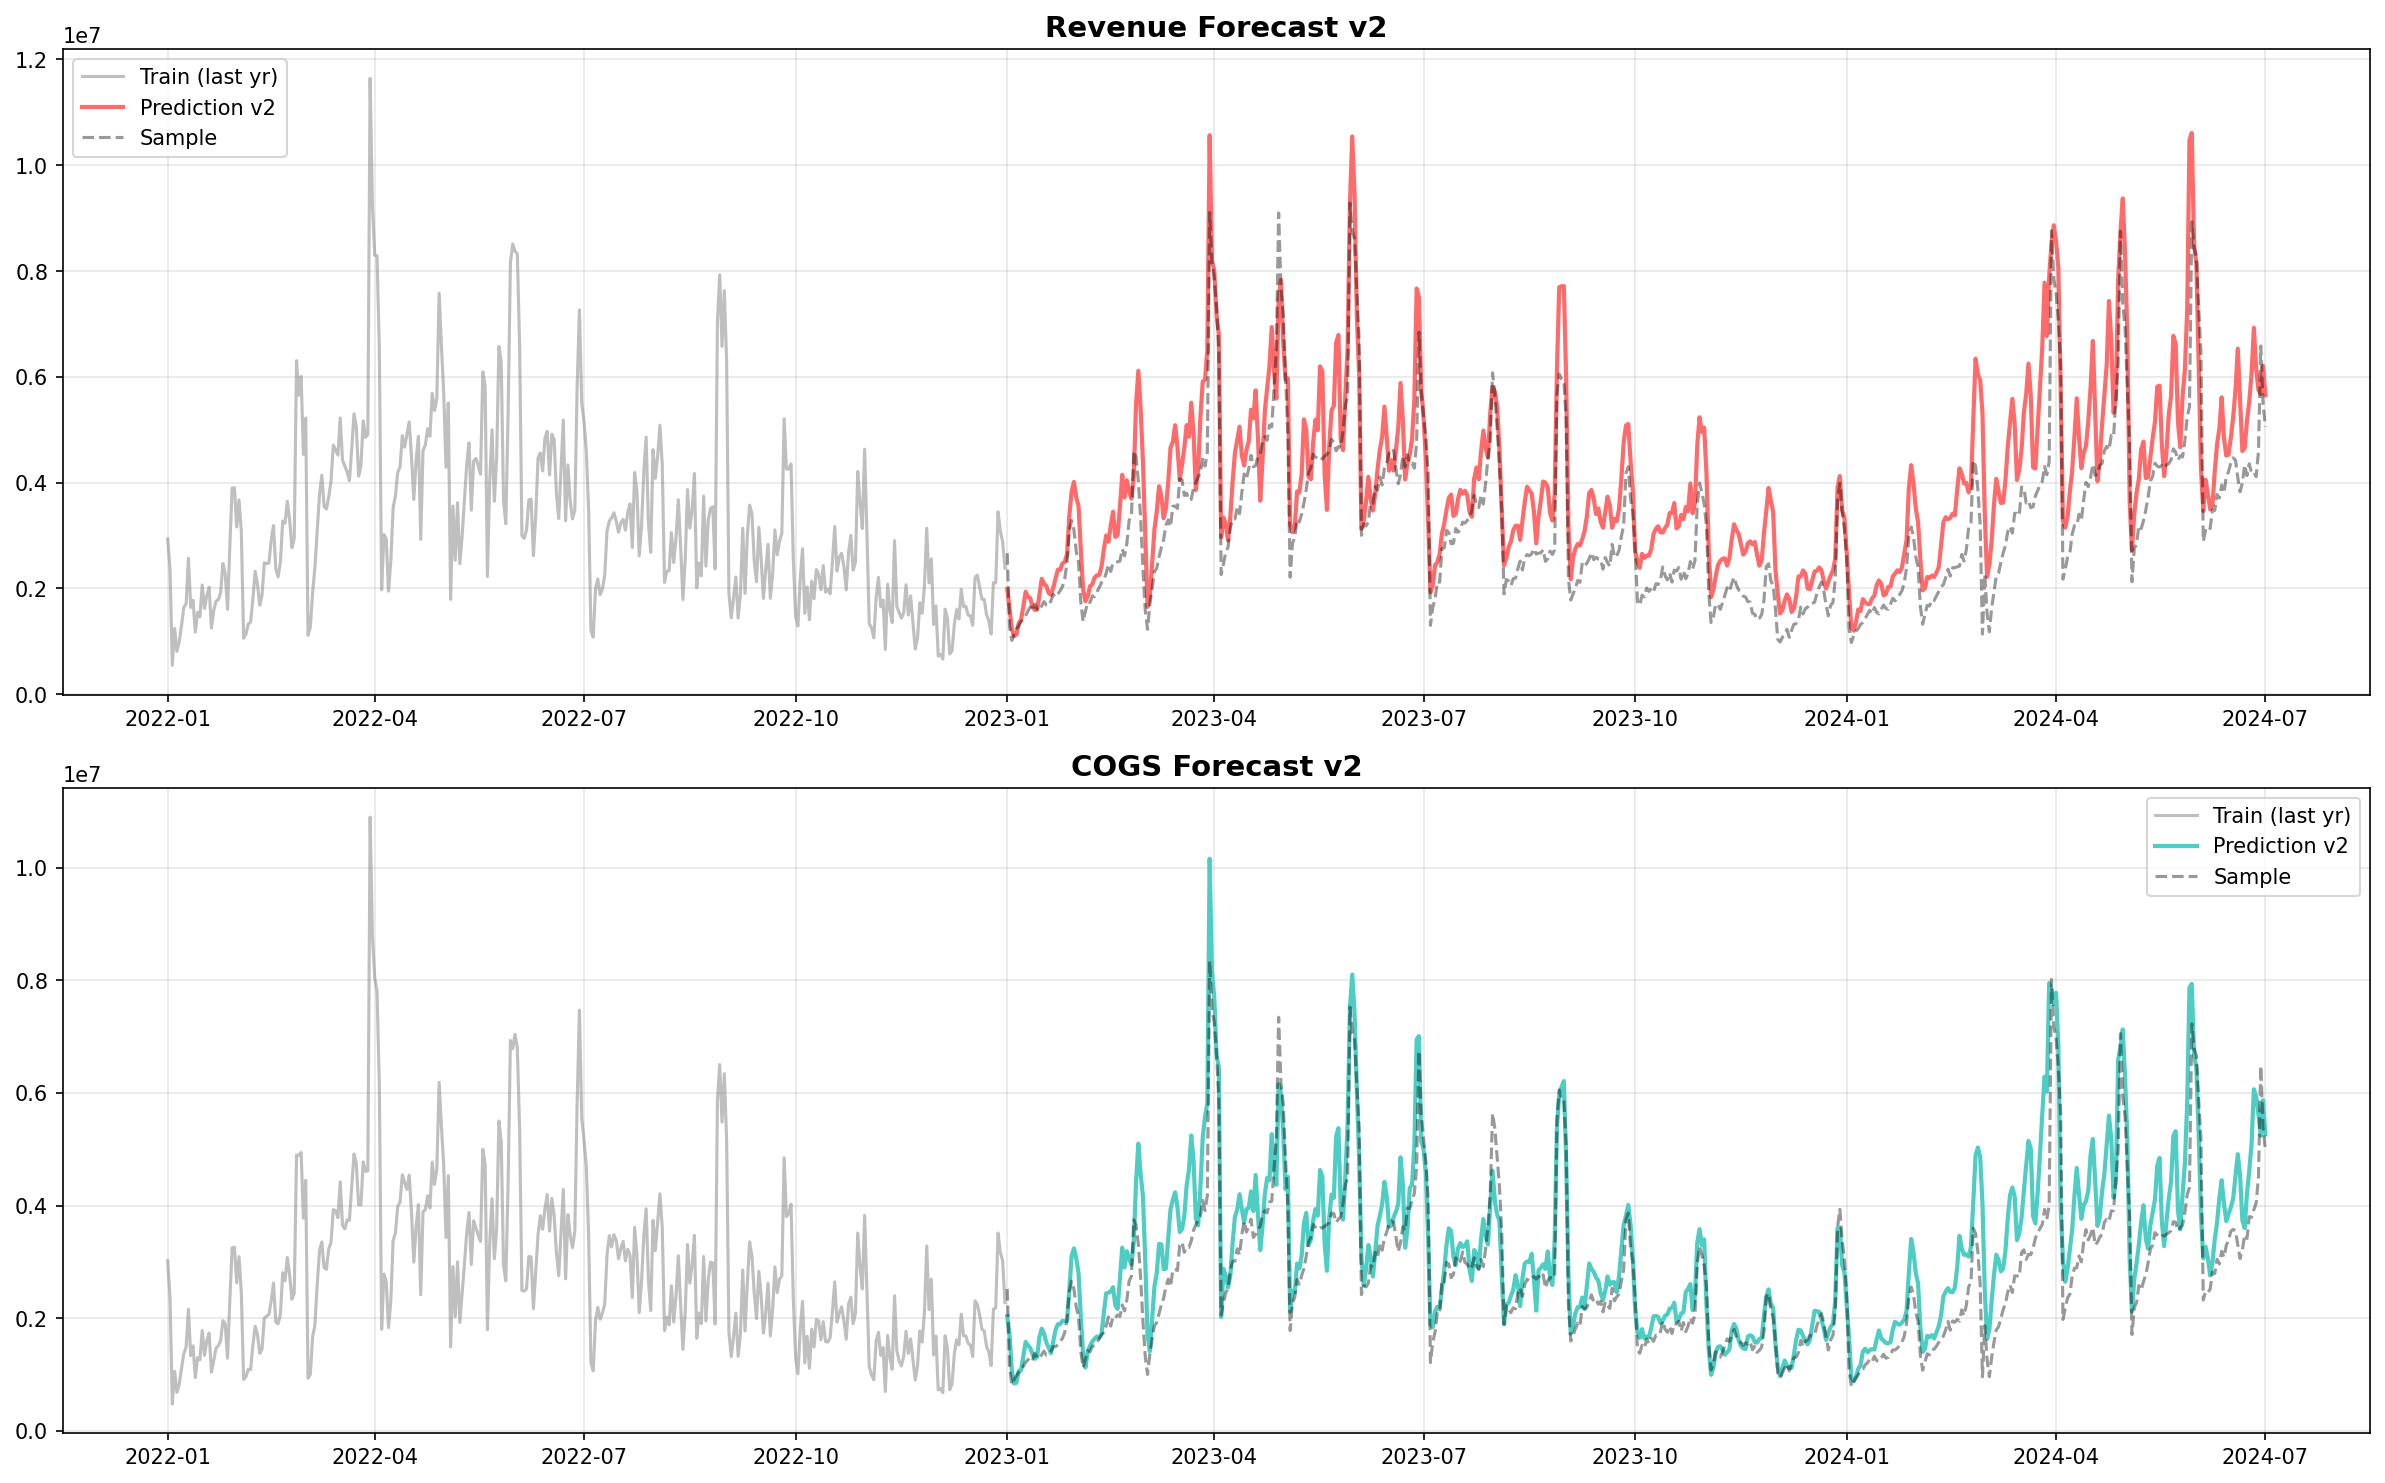
\includegraphics[width=\linewidth]{forecast_v2.png}
    \vspace{-0.5cm}
    \caption{Revenue \& COGS forecast vs.\ training tail}
    \label{fig:forecast}
  \end{subfigure}
  \hfill
  \begin{subfigure}[b]{0.44\linewidth}
    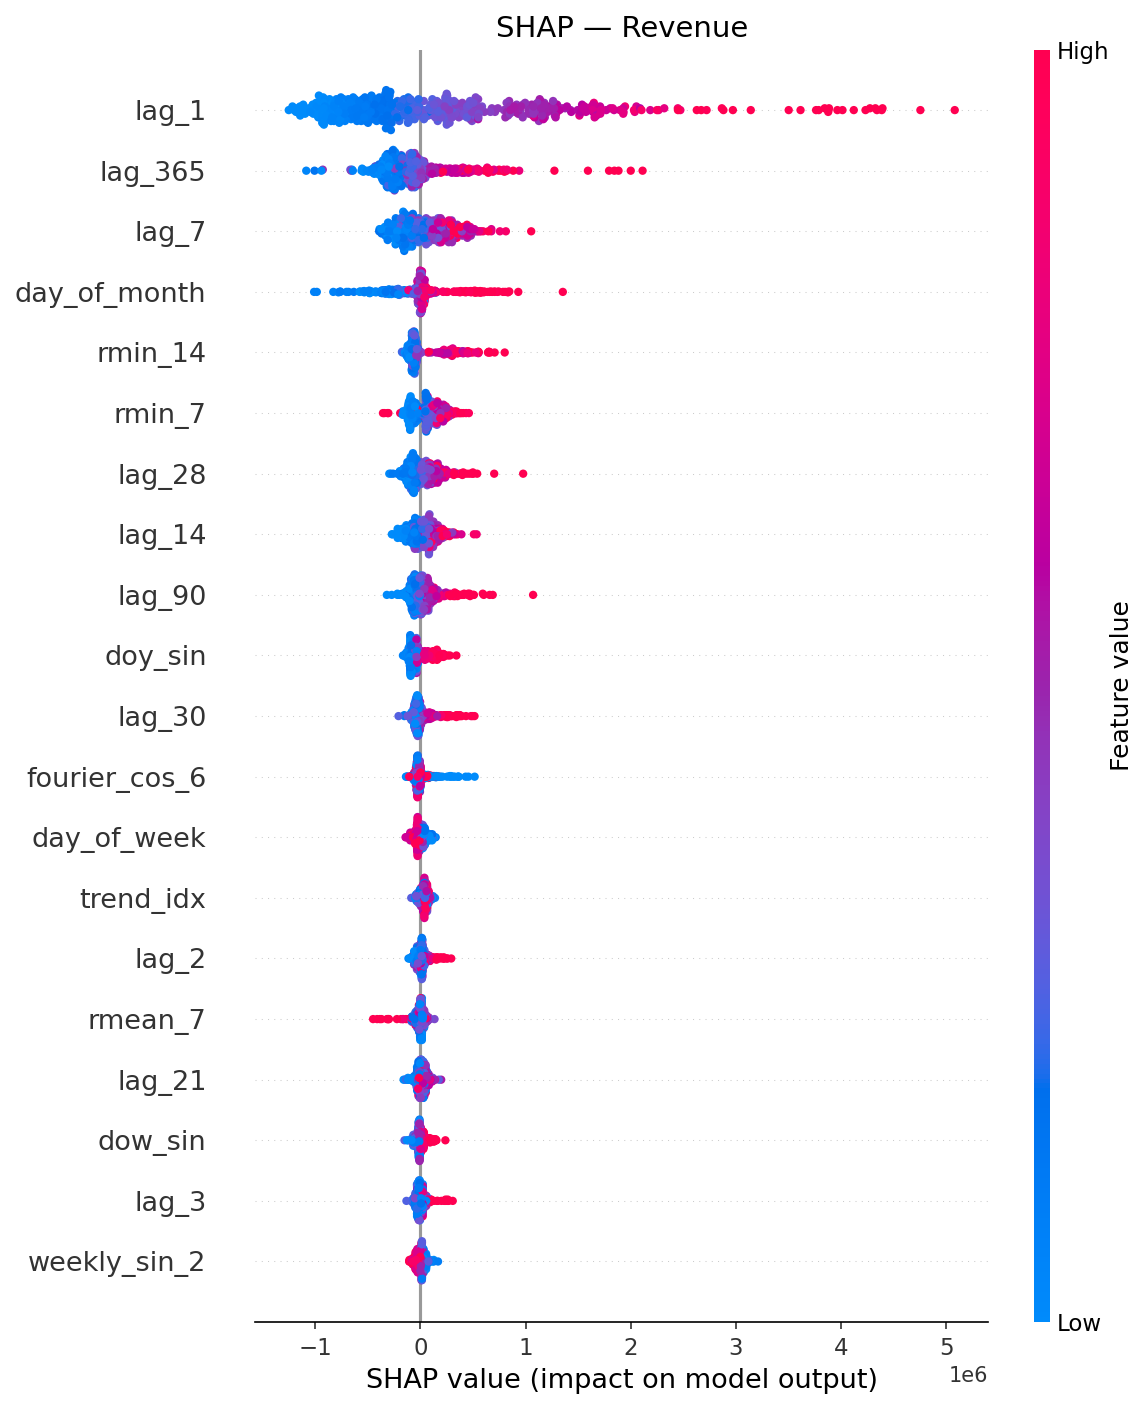
\includegraphics[width=\linewidth]{shap_v2_revenue.png}
    \vspace{-0.5cm}
    \caption{SHAP summary --- Revenue}
    \label{fig:shap}
  \end{subfigure}
  \vspace{-0.1cm}
  \caption{(a)~The ensemble captures weekly and seasonal patterns over 548 days without drift. Dashed line: sample submission baseline. (b)~SHAP confirms lag features and day-of-year cyclical encodings as dominant predictors.}
  \label{fig:results}
\end{figure}

% ==============================================================================
% CONCLUSION
% ==============================================================================
\section{Conclusion}

We present an end-to-end analytics and forecasting solution for Vietnamese e-commerce fashion data. Our four-level EDA reveals that revenue seasonality is traffic-driven (not conversion-driven), customer lifetime value has stagnated due to flat AOV, and nearly 30\% of repeat customers are at high churn risk. Our ensemble forecasting pipeline achieves the best Kaggle score with a deliberately parsimonious feature set, demonstrating that for long-horizon recursive forecasting, simplicity and robustness outperform complexity. Future directions include marketing spend integration for causal attribution, probabilistic forecasting with uncertainty quantification, and real-time churn detection based on the inter-order gap framework.

% ==============================================================================
% REFERENCES
% ==============================================================================
\vspace{-0.1cm}
\section*{References}
\vspace{-0.1cm}

{\footnotesize
\setlength{\parskip}{1pt}

[1] VinTelligence \& VinUniversity DS\&AI Club (2026). Datathon 2026---The Gridbreakers. \url{https://kaggle.com/competitions/datathon-2026-round-1}

[2] Chen, T. \& Guestrin, C. (2016). XGBoost: A Scalable Tree Boosting System. \textit{KDD}, pp.~785--794.

[3] Ke, G. et al. (2017). LightGBM: A Highly Efficient Gradient Boosting Decision Tree. \textit{NeurIPS 30}, pp.~3146--3154.

[4] Prokhorenkova, L. et al. (2018). CatBoost: Unbiased Boosting with Categorical Features. \textit{NeurIPS 31}, pp.~6638--6648.

[5] Lundberg, S.M. \& Lee, S.I. (2017). A Unified Approach to Interpreting Model Predictions. \textit{NeurIPS 30}, pp.~4765--4774.

[6] Pedregosa, F. et al. (2011). Scikit-learn: Machine Learning in Python. \textit{JMLR} 12, pp.~2825--2830.
}

\end{document}
